\documentclass[12pt]{article}
\edef\restoreparindent{\parindent=\the\parindent\relax}
\usepackage{parskip}
\restoreparindent
\usepackage{german}
\usepackage{textcomp}
\usepackage{amsmath}
\usepackage{xcolor}
\usepackage{graphicx}
\usepackage[unicode]{hyperref}

\hypersetup{
    colorlinks = true,
    linkcolor = black,
    linkbordercolor = gray,
    pdfborderstyle={/S/U/W 1},
    urlcolor = blue,
    urlbordercolor = blue
}

\newcommand*{\fullref}[1]{\hyperref[{#1}]{\ref{#1} \nameref{#1}}}   % zeigt die Nummer UND den Namen an


\begin{document}

  \begin{titlepage}

    \begin{center}
      \Huge
  
      HTW-Dresden
  
      Allgemeine Informatik
  
      \bigskip
  
      \LARGE
  
      \vfill
  
      \huge
  
      \textbf{LoRaWAN Wetterstation}
  
      \LARGE
  
      \vfill
  
      Projektseminar\\
      Wintersemester 21/22
  
      \bigskip
  
    \end{center}
  
    \vfill
  
    \Large

  
    \vspace*{2\bigskipamount}
  
    \centering

    \begingroup
      \setlength{\tabcolsep}{12pt}
      \begin{tabular}{lll}
        Name:     & Reitz   & Rezaii-Djafari\\[2.0ex]
        Vorname:  & Lenny   & Raphael\\[2.0ex]
        s-Nummer: & s80452  & s80455
      \end{tabular}
    \endgroup
  
    \vspace*{4\bigskipamount}
  

    Tag der Einreichung: \today
  
    \vspace*{2\bigskipamount}
  
    Professor: Prof. Dr.-Ing. Jörg Vogt 
  
  \end{titlepage}

  \newpage


  \tableofcontents


  \newpage


  \section{Einleitung}
    Das Projekt wurde im Laufe des Projektseminars 2021 von Lenny Reitz und Raphael Rezaii-Djafari unter der Führung von
    Professor Jörg Vogt an der HTW Dresden entwickelt.



    \subsection{Die Übetragungstechnik: LoRa}
      LoRa (Abkürzung für Long Range) ist eine patentierte und proprietäre drahtlose Modulationstechnik basierend auf Chirp Spread Spectrum.
      Seit seiner Veröffentlichung in 2015 durch die \href{www.semtech.com}{Semtech Corporation} hat es sich für
      IoT Geräte bewährt, die außerhalb der konventionellen Reichweiten von W-Lan, Bluetooth und ZigBee operieren.

      Anders als Bluetooth und W-Lan können nur geringe Datenmengen mit niedriger Bitrate gesendet werden,
      dafür aber über eine erheblich größere Reichweite bei geringem Energieverbrauch. LoRa funkt standardmäßig auf dem freien Sub-1-GHz Band,
      weshalb die nutzbaren \href{https://www.thethingsnetwork.org/docs/lorawan/frequencies-by-country/}{Frequenzen}, \href{https://www.thethingsnetwork.org/docs/lorawan/duty-cycle/}{Fair-Use-Policies}
      und Vorschriften am Einsatzort beachtet werden müssen. Für eine höhere Datenrate und keine Beschränkungen gibt es auch eine
      \href{https://www.semtech.com/products/wireless-rf/lora-24ghz}{Variante mit 2.4GHz} auf die wir nicht weiter eingehen.



    \subsection{Das Protokoll \& die Architektur: LoRaWAN}
      LoRaWAN wird Open Source von der \href{https://lora-alliance.org/}{LoRa Alliance} als Systemarchitektur und Netzwerkprotokoll
      auf der Vermittlungsschicht entwickelt.

      \subsubsection{Systemarchitektur}
        Vermaschte Netze werden genutzt um eine große Abdeckung kosteneffizient zu erzielen, allerdings steht der Stromverbrauch durch die Komplexität und das
        Weiterleiten der Pakete durch die Geräte, ab hier Endknoten genannt, im Widerspruch zur geforderten Energieeffizienz der Endknoten.
        Da LoRa onehin eine große Reichweite besitzt, wird eine Stern-Topologie verwendet.

        Netzwerkknoten stehen dabei nicht für ein einzelnes, sondern für
        eine beliebig große Anzahl geographisch naher Gateways. Wenn ein Endknoten Daten sendet, passiert dies durch Broadcasts.
        Alle Gateways, die das Paket erhalten haben, senden es an den Netzwerk Server, der redundante Pakete herausfiltert,
        Sicherheitschecks durchführt und schließlich das Paket an seinen Bestimmungsort weiterleitet.

        \begin{figure}[h!]
          \center
          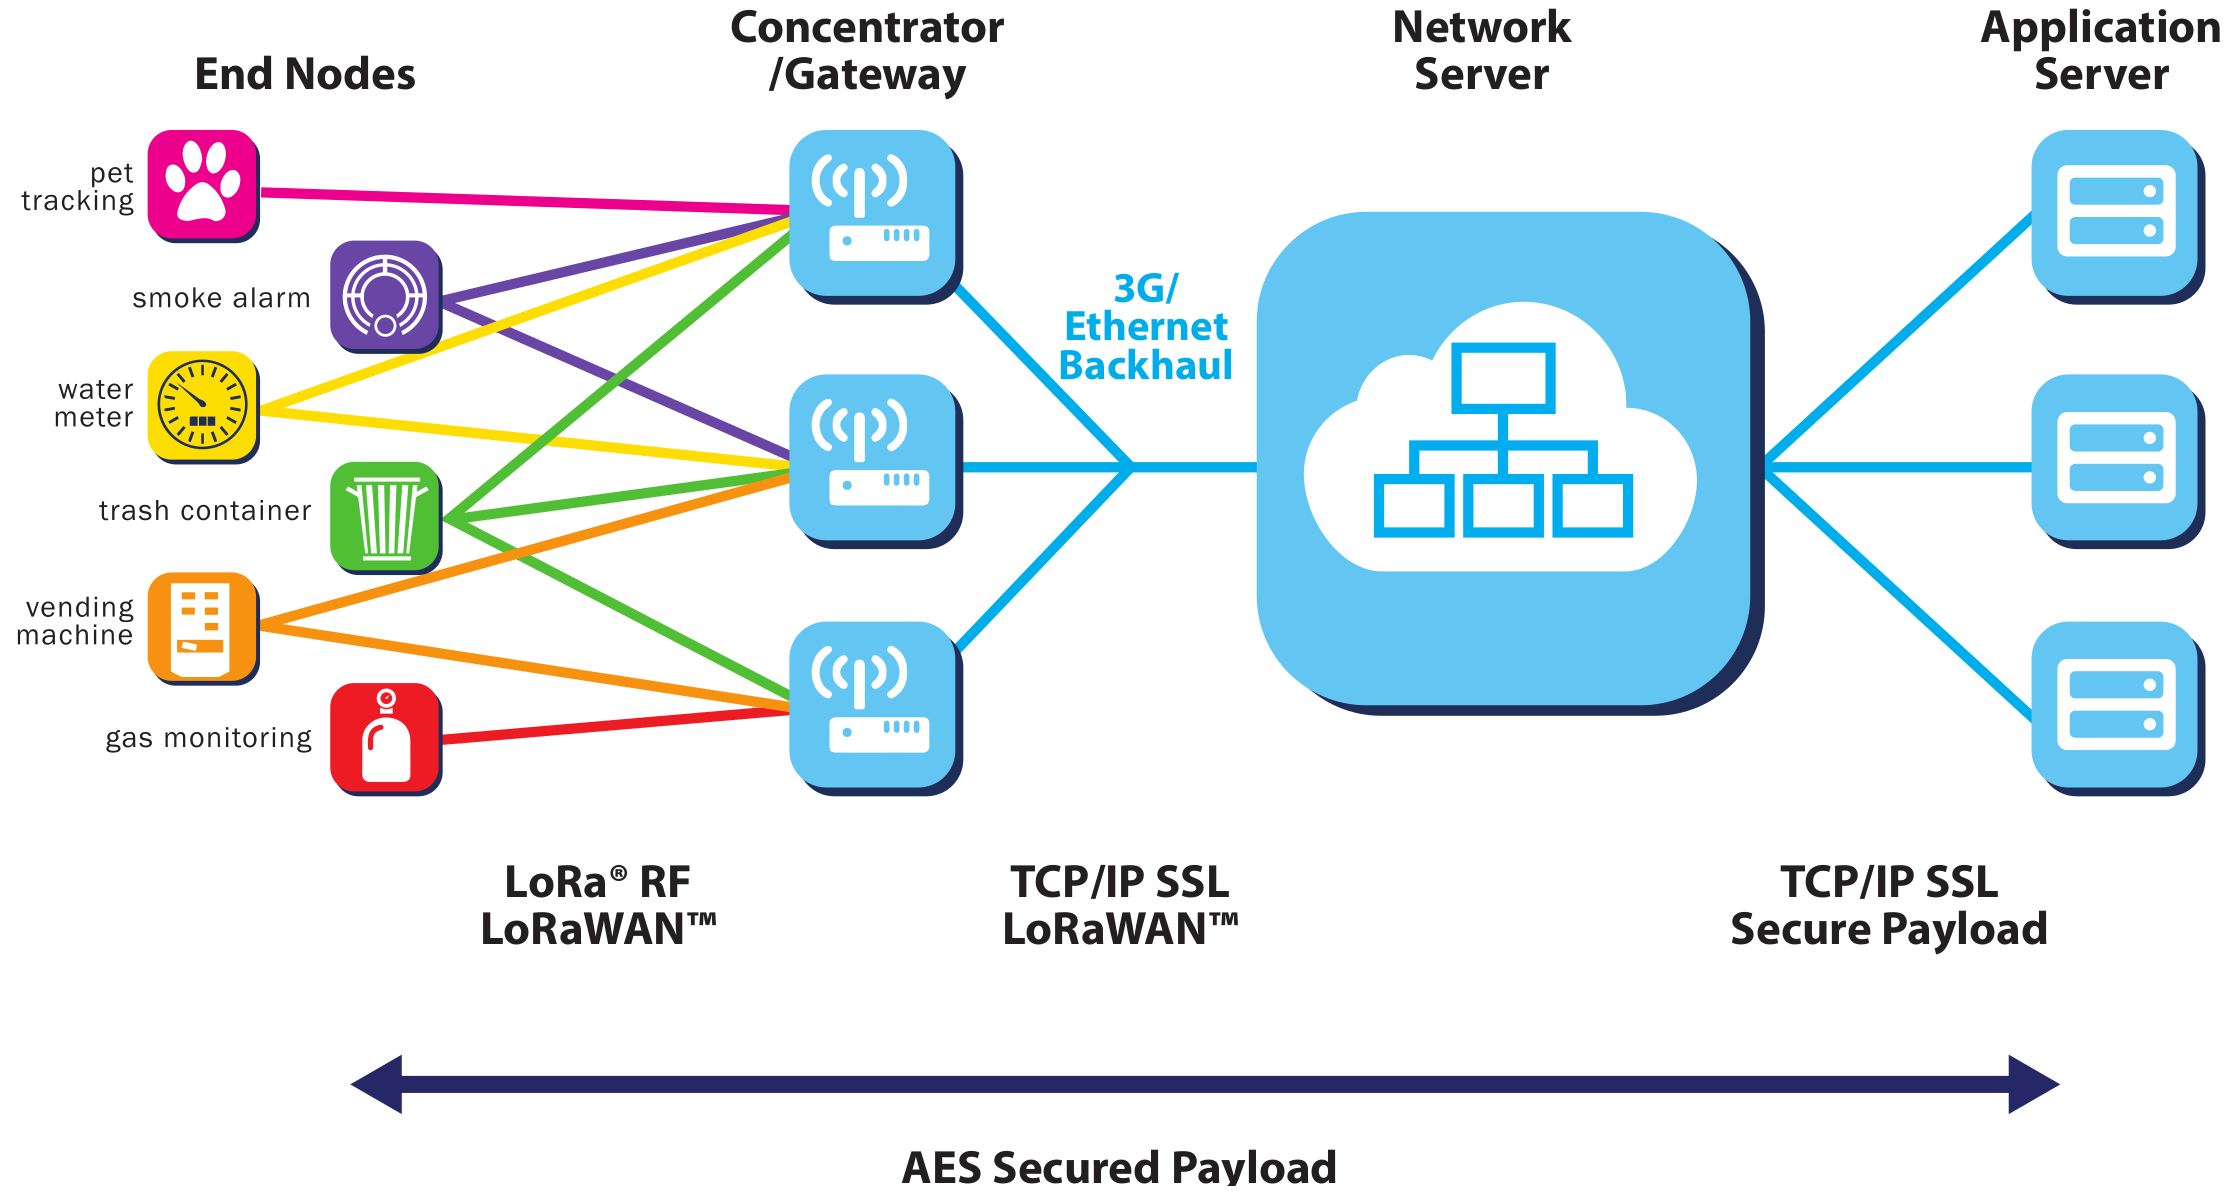
\includegraphics[scale = 0.17]{./img/LoRaWAN_Systemarchitektur.png}
          \caption{LoRaWAN Architektur\protect\footnotemark[1]}
        \end{figure}

        Dadurch verlagert sich die Komplexität von den Endknoten und Gateways auf den Netzwerk Server.
        Außerdem wird die Verfügbarkeit verbessert, wenn ein Gateway ausfällt oder ein Endknoten mobil ist, da kein Handover notwendig ist.\footnotemark[1]

        \footnotetext[1]{LoRa Alliance. (2015). A technical overview of LoRa and LoRaWAN [Ebook] (pp. 7-9). \href{https://lora-alliance.org/wp-content/uploads/2020/11/what-is-lorawan.pdf}{https://lora-alliance.org/wp-content/uploads/2020/11/what-is-lorawan.pdf}}
    

      
      \subsubsection{Geräteklassen}
        Nicht jedes IoT Gerät hat die gleichen Anforderungen. Generell gilt, dass die Kommunikation bidirektional, asynchron und verschlüsselt erfolgt, wobei Endknoten Daten zum Netzwerk senden
        sobald diese verfügbar sind. Der Unterschied zwischen den Klassen liegt darin, wann ein Endknoten Daten vom Netzwerk empfangen kann.

        \begin{itemize}
          \item \textbf{A: batteriebetriebene Sensoren}
          \item[] Ein Empffangsfenster wird nur geöffnet nachdem Daten an das Netzwerk übertragen wurden. Das Netzwerk muss Downlink Kommunikation
            für das Gerät solange bereithalten bis dieses Daten sendet. Klasse A ist am energiesparsamsten und muss von allen Geräten unterstützt werden.
          \item \textbf{B: batteriebetriebenes Steuergerät}
          \item[] Zusätzlich zu den Eigenschaften der Klasse A, öffnen Geräte der Klasse B das Empfangsfenster zu festgelegten Zeiten. Eine zeitliche Synchronisation mit dem Gateway ist erforderlich.
          \item \textbf{C: Steuergerät mit fester Stromversorgung}
          \item[] Das Empfangsfenster der Geräte der Klasse C ist permanent geöffnet. Es wird nur bei Übertragungen geschlossen.
        \end{itemize}

      

      \subsubsection{LoRaWAN Netzbetreiber} \label{subsec:LoRaWAN Netzbetreiber}
        Aufgrund der Open Source Natur von LoRaWan gibt es die verschiedensten Netzbetreiber. Wir werden uns auf das populäre
        \href{https://www.thethingsnetwork.org/}{The Things Network / The Things Stack} (TTN) beschränken.
        Es ist frei nutzbar, allerdings gibt es neben den Frequenzrichtlinien, keine Uptime Verpflichtungen und eine \href{https://www.thethingsnetwork.org/docs/lorawan/duty-cycle/}{Fair-Use-Policy}:

        \begin{itemize}
          \item Die Uplink Airtime (Endknoten \textrightarrow{} TTN) ist auf 30 Sekunden je 24 Stunden pro Endknoten beschränkt.
          \item Es dürfen maximal 10 Downlink Nachrichten (TTN \textrightarrow{} Endknoten) je 24 Stunden pro Endknoten gesendet werden.
        \end{itemize}
        
        Für die nachfolgende \underline{\nameref{subsec:Problemstellung}} eignet sich das TTN optimal. Es sei jedoch erwähnt, dass das kommerzielle \href{https://www.thethingsindustries.com/}{The Things Industries} (TTI) mit weniger Beschränkungen und SLAs existiert.
         


    \subsection{Problemstellung} \label{subsec:Problemstellung}
        Wir haben eine analoge Wetterstation und wollen diese an das TTN anbinden.
        Dafür nutzen wir einen Arduino Uno mit LoRa Shield.

        Die Wetterstation muss verbunden und ein Programm geschrieben werden, dass die Daten ausließt und versendet.
        Die Auflösung und Anzahl der Datensätze, sowie Übertragungsparameter, Authentifizierungsmethoden und Schlüssel
        müssen einfach konfigurierbar sein.



  \section{Aufbau/Übersicht}

    \subsection{Hardware}

      \begin{itemize}
        \item\href{https://learn.sparkfun.com/tutorials/weather-meter-hookup-guide#resources-and-going-further}{Wettermessgerät-Kit} SEN-15901
        
        \begin{itemize}
          \item beinhaltet Regenmesser, Anemometer, Windfahne
        \end{itemize}

        \item Breadboard
        \item Jumper-Kabel
        \item 10 kOhm Widerstand
        \item 2 \href{https://www.pollin.de/p/modular-einbaubuchse-mit-anschlusslitzen-6p6c-541843}{Modular-Einbaubuchsen mit Anschlusslitzen, 6P6C}
        \item Arduino Uno
        \item \href{https://wiki.dragino.com/index.php?title=Lora_Shield}{Dragino Lora Shield v1.4}
      \end{itemize}

      \subsubsection{Aufbau}

    \subsection{Software}

      \subsubsection{Libraries}
    
      TODO - LoRa Library



  \section{Funktionsweise}

    \subsection{TTN}
      Wie schon in \underline{\fullref{subsec:LoRaWAN Netzbetreiber}} genannt nutzen wir das The Things Network.
      Zur Verwaltung der Applications (Verbund von Endknoten) und Gateways gibt es die Console.

      In dieser lassen sich Applications und Gateways erstellen, aktuelle Daten anzeigen und Einstellungen konfigurieren.
      Besonders für Endknoten interessant sind der Payload Formatter, Integrations und ADR.

      \begin{itemize} %TODO: evtl in subsubsectionen ausgliedern
        \item \textbf{Payload Formatter}
        \item[] In diesem lassen sich Uplink und Downlink Nachrichten umwandeln.
          Bei der Übertragung über LoRa sollte die Payload stets so klein wie möglich sein, weshalb die Daten als Bits/Bytes kodiert werden.
          Siehe dazu auch \href{https://www.thethingsnetwork.org/docs/devices/bytes/}{Working with Bytes}.
          Damit das TTN die Payload definiert in X interpretieren kann müssen wir einen Payload Formatter setzen. Sieh %TODO: Verlinkung zu Definition der Payload
        \begin{itemize}
          \item Das Setzen eines Payload Formatter wird in \underline{\ref{subsec:Payload Formatter setzen}} beschrieben.
        \end{itemize}
        \item \textbf{Integrations}
        \item[] Hier gibt es die Möglichkeit Trigger zu erstellen die Daten verarbeiten und weiterleiten.
          Beispielsweise Webhooks oder Storage Integrations für Up- und Downlink Nachrichten.
          Für eine Auflistung siehe \href{https://www.thethingsnetwork.org/docs/applications-and-integrations/}{Applications \& Integrations}.
        \item \textbf{Adaptive Data Rate - ADR}
        \item[] \href{https://www.thethingsnetwork.org/docs/lorawan/adaptive-data-rate/}{ADR} ist ein Mechanismus für Endknoten
        der Spreading Factor, Datenübertragungsrate und Sendeleistung optimiert. Dafür werden die letzten 20 Uplink Nachrichten analysiert.
        Es ist standardmäßig für jeden Endknoten aktiviert, sollte für mobile Endknoten jedoch deaktiviert werden. Siehe \underline{\fullref{subsec:ADR deaktivieren}}.
      \end{itemize}



    \subsection{Authentifizierungsmethoden} \label{subsec:Authentifizierungsmethoden}
      Um einen Endknoten im TTN zu Authentifizieren gibt es zwei Möglichkeiten. Beim Anlegen des Endknotens in der TTN Console muss entweder
      OOTA oder ABP gewählt werden, wobei OOTA vorzuziehen ist.

      Einen wichtigen Aspekt spielt dabei im Bezug auf Sicherheit der Frame Counter. Mit jedem gesendeten Paket wird dieser inkrementiert
      und vom Netzwerk verifiziert um Replay Attacken zu verhindern.

      \subsubsection{Over-the-Air Activation - OOTA}
        Bei der bevorzugten Variante OOTA wird ein Join Verfahren beim Einschalten des Endknotens initialisiert,
        wobei Identifikationsinformationen, inklusive Frame Counter, und Schlüssel ausgetauscht werden. Ebenso werden die verfügbaren Frequenzen und
        der optimale Spreading Factor ermittelt.

      \subsubsection{Activation by Personalization - ABP}
        Bei ABP werden die vordefinierten Identifikationsinformationen, Spreading Factor und Schlüssel auf dem Gerät gespeichert.
        Falls ADR deaktiviert ist, bleibt der Spreading Factor konstant. Da es kein Join Procedure gibt, muss der Frame Counter,
        persistent abgespeichert werden. Der Arduino Uno besitzt aber keinen persistenten Speicher. Wenn dieser nun ausgeschaltet wird, resettet sich der Frame
        Counter auf 0 und beim erneuten Anschalten werden alle Pakete vom TTN verworfen. 

        \textit{Hinweis:} Der Arduino Uno besitzt ein EEPROM welchen man nutzen könnte um den Frame Counter zu speichern. Dieser hat jedoch eine begrenzte
        Lebensdauer von ungefähr 100,000 Schreibzyklen.\footnote[2]{Egger, Alexander. Arduino und der EEPROM. Retrieved 10 February 2022, from \href{https://www.aeq-web.com/arduino-atmega-eeprom-read-write-details/}{https://www.aeq-web.com/arduino-atmega-eeprom-read-write-details/}}
        Der Versuch den Frame Counter im RAM zu behalten und nur beim Ausschalten zu speichern funktioniert nicht, da bei einem Stromausfall
        die Operation nicht durchgeführt wird. Um das zu umgehen kann mit jedem gesendeten Paket der EEPROM beschrieben werden. Dann ist dieser nach
        spätestens 100,000 Paketen nicht mehr beschreibbar, was abhängig vom Sendeinterval schnell sein kann.

        Daher empfehlen wir unbedingt OTAA. Sollte man dennoch ABP nutzen wollen, so lässt sich in der TTN Console die Frame Counter Überprüfung deaktivieren,
        wie gezeigt in \underline{\fullref{subsec:ABP-Konfiguration}}, wodurch Replay Attacken nicht mehr verhindert werden.

        %TODO: Problem mit Frequenzen ansprechen

    \subsection{Sensoren der Wetterstation}

      \subsubsection{Regenmesser}

        Der Regenmesser besteht aus einem Auffangbehälter und einem darin befindlichen einfachen Kippschalter.
        Wenn sich genügend Wasser im Behälter gesammelt hat, kippt der Schalter um und das Wasser läuft wieder aus dem Behälter heraus.
        Ein Kippvorgang entspricht einer Wassermenge von 0,2794 mm.
        Die folgende Umrechung ergibt die Wassermenge in Milliliter bei einer Auffangfläche von 55 cm²:

        \begin{multline}
          1\,mm = 1\,l/m^2 \quad \text{(Niederschlag)} \\
          \Rightarrow 0.2794\,mm = 0.2794\,l/m^2 = 0.02794\,ml/cm^2 \\
          \Rightarrow 0.02794\,ml/cm^2 * 55\,cm^2 \approx 1.54\,ml
        \end{multline}

        Ein Kippen beträgt also im Idealfall 1,54 ml. Mehrere Testläufe haben aber gezeigt, dass der Regenmesser mit einer relativ großer Ungenauigkeit schaltet.
        Je nach dem, wie schnell das Wasser einfließt, variiert die Messgenauigkeit stark.

      \subsubsection{Anemometer}

        Das Schalenanemometer misst Windgeschwindigkeiten durch Schließen des Kontaktes eines Schalters durch einen Magneten.
        Eine Windgeschwindigkeit von 2.4 km/h schließt den Schalter einmal pro Sekunde.

        Eine Umdrehung entspricht 3 Schaltvorgängen.

      \subsubsection{Windfahne}

        Die Windfahne besitzt 8 Schalter, welche jeweils mit unterschiedlich großen Widerständen verbunden sind.
        Die Schalter könne einzeln oder in Paaren umgelegt werden, wodurch sich 16 mögliche Positionen bestimmen lassen.

        Durch einen externen Widerstand wird ein Spannungsteiler implementiert, der eine messbare Spannung ausgibt.
        Daher lässt sich die Windrichtung nur durch ein analoges Signal bestimmen.

    \subsection{Beispielablauf}

      Benötigte Payload Größe (pro Sekunde):

      \begin{itemize}
        \item Windfahne: 4 Bit (16 mögliche Windrichtungen)
        \item Regenmesser: 2 Bit (maximal 4 Klicks pro Sekunde)
        \item Anemometer: 7 Bit (maximal 128 Klicks pro Sekunde)
      \end{itemize}

      => 13 Bit Payload Größe (pro Sekunde)
      Wenn wir 60 Messwerte pro Minute aufnehmen würden und dann pro Minute diese Daten an das TTN senden würden, bedeutet das:

      \begin{itemize}
        \item Payload Größe: 13 Bit * 60 = 780 Bit ~ 98 Byte (pro Minute)
      \end{itemize}

      Es muss eine Konfiguration für LoRa eingestellt werden, welche optimal für die zu sendende Paketgröße und Sendeinterval abgestimmt ist.

      Laut https://www.thethingsnetwork.org/airtime-calculator ist die minimale Airtime für unsere Paketgröße und Sendeinterval:

      \begin{itemize}
        \item Paketgröße: 98 Byte
        \item Spreading Factor: SF7
        \item Region: EU868
        \item Bandbreite: 250 kHz
      \end{itemize}

      => Airtime: 94,8 ms

      Problem, weil die Fair Use Policy von TTN nur 30s Airtime pro Tag erlaubt. Wir sind allerdings mit 137s pro Tag weit darüber.

      => Eine rohe Übermittlung der Daten mit einer Genaugikeit von 1s ist nicht möglich.

      Schlussfolgerung: Die Rohdaten müssen gemittelt werden, um eine Übertragung innerhalb der 30s pro Tag zu einzuhalten.

      
      pro 5 Sekunden:

      - Regenmesser: 3 Klicks * 5 Sekunden = 15 Klicks => 4 Bits
      - Anemometer: Wert wird gemittelt => 7 Bits
      - Windfahne: Wert wird gemittelt => 4 Bits

      => Gesamt: 15 Bits pro 5 Sekunden

      => Pro Minute: 180 Bits ~ 23 Byte


      pro 10 Sekunden:

      - Regenmesser: 3 Klicks * 10 Sekunden = 30 Klicks => 5 Bits
      - Anemometer: Wert wird gemittelt => 7 Bits
      - Anemometer: Maximalwert => 7 Bits
      - Windfahne: Wert wird gemittelt => 4 Bits

      => Gesamt: 23 Bits pro 10 Sekunden

      => Pro Minute: 138 Bits ~ 18 Byte

      => pro 5 Minuten: 690 Bits ~ 87 Byte

      Das wäre eine mögliche Konfiguration mit einer Airtime von 87.2 ms pro 5 Minuten oder 25.1 s pro Tag
  
      

  \section{Konfiguration \& Verbindung der Wetterstation}
    In dieser Dokumentation wird nicht darauf eingegangen wie ein Gateway eingerichtet wird.
    Konsultieren Sie dafür die Betriebsanleitung des Herstellers.

    \textbf{Vorbedingung:}
    \begin{enumerate}
      \item Installieren Sie die Arduino IDE und die notwendige \href{https://github.com/dragino/arduino-lmic}{Library} nach \texttt{Installation.md}
      \item Erstellen Sie einen TTN Account unter \href{www.thethingsnetwork.org}{www.thethingsnetwork.org}
      \item Navigieren Sie zur Console
      \item Wählen Sie \textless Go to applications\textgreater{}
      \item Fügen Sie durch \textless Add application\textgreater{} eine Application hinzu
      \item Wählen Sie \textless Add end device\textgreater{} und wechseln in den \textless Manually\textgreater{} Tab
      \item Frequency Plan: Europe 863-870 MHz (SF9 for RX2 - recommended)
      \item LoRaWan version: MAC V1.0.2
      \item Regional Parameters version: PHY V1.0.2 REV A
    \end{enumerate}
    
    Wie bereits in \underline{\fullref{subsec:Authentifizierungsmethoden}} erläutert, empfehlen wir OTAA gegenüber ABP.



    \subsection{OTAA-Konfiguration}
      \begin{enumerate}
        \setcounter{enumi}{9}
        \item DevEUI: Generate
        \item AppEUI: Fill with zeros
        \item AppKey: Generate
        \item \textless Register end device \textgreater{}
        \item Wechseln Sie zu \texttt{secret.template.h} und geben Sie die generierten Daten ein.
          Achten Sie ggf. auf das little-endian Format.
        \item Benennen Sie \texttt{secret.template.h} in \texttt{secret.h} um
        \item Öffnen Sie \texttt{config.h} und aktivieren Sie den OTAA Modus
        \item Wählen Sie Ihre gewünschten Datenauflösung und die Größe der Payload.
          Betrachten Sie dazu das Beispiel, verifizieren Sie die Größe der Payload mit dem
          \href{https://www.thethingsnetwork.org/airtime-calculator}{LoRaWAN airtime calculator}
        \item Prüfen Sie, dass die \href{https://www.thethingsnetwork.org/docs/lorawan/duty-cycle/}{Fair-Use-Policy} nicht verletzt wird
        \item Beachten Sie, dass bei OTAA der Spreading Factor automatisch gesetzt wird.
          Wählen Sie am besten Werte die mit SF12 noch Fair-Use sind.
        \item Falls gewünscht, können Sie \underline{\nameref{subsec:ADR deaktivieren}}.
        \item Installieren Sie das Programm auf dem Arduino Uno.
        \item Machen Sie weiter mit \underline{\nameref{subsec:Payload Formatter setzen}}.
      \end{enumerate}



    \subsection{ABP-Konfiguration} \label{subsec:ABP-Konfiguration}
      \begin{enumerate}
        \setcounter{enumi}{9}
        \item \textless Show advanced activation, LoRaWAN class and cluster settings \textgreater{}
        \item Activation mode: ABP
        \item DevEUI: Generate
        \item Device address: Generate
        \item AppSKey: Generate
        \item NwkSKey: Generate
        \item \textless Register end device \textgreater{}
        \item Nachfolgend deaktivieren Sie den Frame Counter, siehe Problematik in \underline{\fullref{subsec:Authentifizierungsmethoden}}.
        \item Wechseln Sie in den \textless General settings\textgreater{} Tab
        \item Wählen Sie bei Network layer \textless Expand\textgreater{}
        \item Wählen Sie unten \textless Advanced MAC settings\textgreater{}
        \item Setzen Sie das Häkchen in \textless Resets frame counters\textgreater{}
        \item Falls gewünscht, entfernen Sie das Häckchen bei \textless Use adaptive data rate (ADR)\textgreater{}
        \item \textless Save changes\textgreater{}
        \item Wechseln Sie zu \texttt{secret.template.h} und geben Sie die generierten Daten ein.
        \item Benennen Sie \texttt{secret.template.h} in \texttt{secret.h} um
        \item Öffnen Sie \texttt{config.h} und aktivieren Sie den ABP Modus
        \item Wählen Sie Ihre gewünschten Datenauflösung und die Größe der Payload.
          Betrachten Sie dazu das Beispiel, verifizieren Sie die Größe der Payload mit dem
          \href{https://www.thethingsnetwork.org/airtime-calculator}{LoRaWAN airtime calculator}
        \item Prüfen Sie, dass die \href{https://www.thethingsnetwork.org/docs/lorawan/duty-cycle/}{Fair-Use-Policy} nicht verletzt wird.
        \item Falls gewünscht, können Sie \underline{\nameref{subsec:ADR deaktivieren}}.
        \item Installieren Sie das Programm auf dem Arduino Uno.
        \item Machen Sie weiter mit \underline{\nameref{subsec:Payload Formatter setzen}}.
      \end{enumerate}



    \subsection{Payload Formatter setzen} \label{subsec:Payload Formatter setzen}
      \begin{enumerate}
        \item Wählen Sie den \textless Payload formatters\textgreater{} Tab
        \item Uplink ist standärdmäßig ausgewählt
        \item Formatter type: Javascript
        \item Kopieren Sie den Javascript Code von \texttt{payload\_formatter.js} in das vorgesehene Feld
        \item \textless Save changes\textgreater{}
        \item Testen Sie den Formatter mit der Payload X %TODO: add payload
        \item Starten Sie den Arduino. Falls ein Gateway in Reichweite ist, sollten die Daten nach einiger
          Zeit im Tab \textless Live data\textgreater{} erscheinen
      \end{enumerate}


    \subsection{ADR deaktivieren} \label{subsec:ADR deaktivieren}
      \begin{enumerate}
        \item Wechseln Sie in den \textless General settings\textgreater{} Tab im TTN
        \item Wählen Sie bei Network layer \textless Expand\textgreater{}
        \item Wählen Sie unten \textless Advanced MAC settings\textgreater{}
        \item Entfernen Sie das Häkchen in \textless Use adaptive data rate (ADR)\textgreater{}
        \item \textless Save changes\textgreater{}
      \end{enumerate}

  \section{Probleme}

\end{document}